\section{Conclusion, Limitations and Future Work}

In this paper, we present a skeleton-based approach for partitioning a shell model into parts which are free of support structure when fabricated. We prove the NP-hardness of the problem. We formulate the model partition problem as a constrained graph partition problem which is particularly tailored toward fabrication. To tackle the NP-hardness of the problem, we exploit a stochastic method which adaptively searches for better partition results while avoiding local minima. We also propose a polynomial time algorithm for the skeleton partition problem. Compared with existing partition-based methods, the advantages of our partition method are as follows:

\begin{itemize}
 \item The models are support-free, especially for the 3D printing techniques including SLA, SLM and SLS. For FDM technique, it requires a bed of support that consumes very little volume of materials.
\item The seams on the assembled model are minimized in terms of cut number and cut length.
\end{itemize}

The support-free feature of our partition approach saves a significant amount of time and printing material both inside and outside of a shell model. Our method is efficient and applicable to a large set of natural and man-made models.

\textbf{Limitations and Future Work.} Our approach is devoted to shell models, it can also be applied to cutting solid models without any problem. However, our approach suffers from a few limitations:
(i) For shell models, the thickness of the shells need to be large enough such that no serious deformation is caused during the assembling process. In this work, we restrict our focus to a uniform setting of the shell thickness whose value is determined by an error-and-trial process. A future research would be to determine the minimum shell thickness in different parts of a given model, this process requires an efficient detection of self-intersection and an experimental study of the printability according to the curvature changes of the shell model.
%(ii) The strength guarantee is not elaborated in this work, a possible solution is to use the algorithm in \cite{WangWYLTTDCL13} that distributes the least amount of materials for constructing a truss frame beneath the skin.
(ii) Our approach may allow a cut that passes through a salience region, which may hurt the appearance of the model. We found that it is difficult to make a balance between the saliency and the minimal cutting length as well as the minimal cutting numbers. A potential future research is to take care of salience region during graph partition; particularly, as a trade-off between support material and salience preservation, a spatially curved cut might be a consideration to alleviate the salience problem.
(iii)  {\color{red} {For a model with tiny spikes that result in local minimum points, a skeleton may not be able to capture the geometric feature of these spikes, which could beg for a support below each local minimum point. Refer to Figure \ref{fig:limit} for an illustration. }}

\begin{figure}[t!]
  \centering
  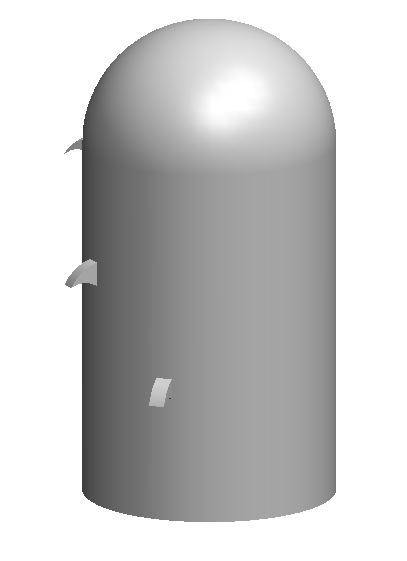
\includegraphics[width=0.2\linewidth]{figs/limit.png}
  \caption{\label{fig:limit}%
  A model with tiny spikes that result in local minimum points.}
\end{figure}



\begin{figure}[t]
  \centering
  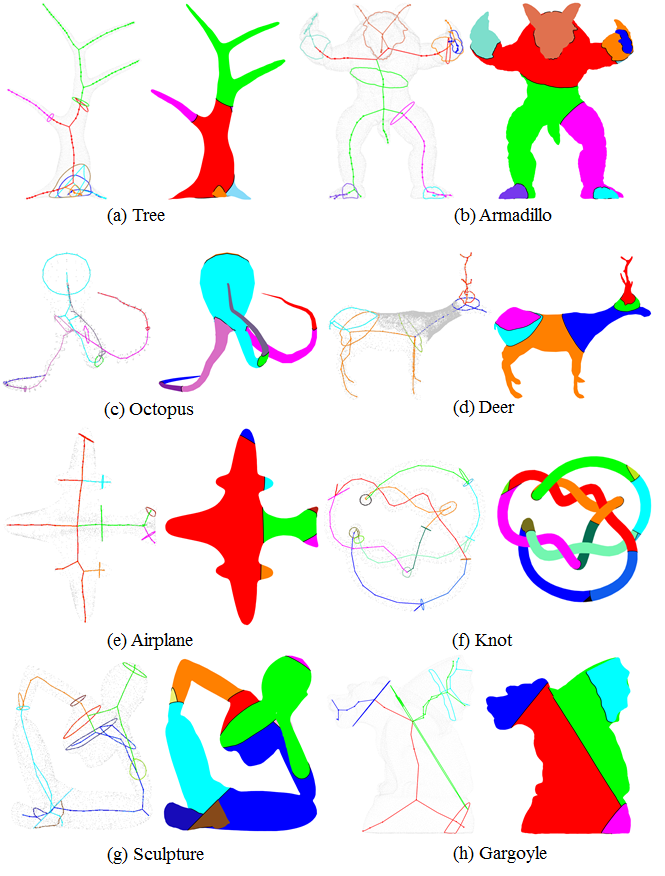
\includegraphics[width=0.3\textwidth]{figs/programming.png}
  \caption{\label{fig:programming}%
           Partition examples as $\theta = 70^{\circ}$. The printing direction of each part is orthogonal to its base (shown in the same color as the part)}
\end{figure}

\begin{figure}[t]
  \centering
  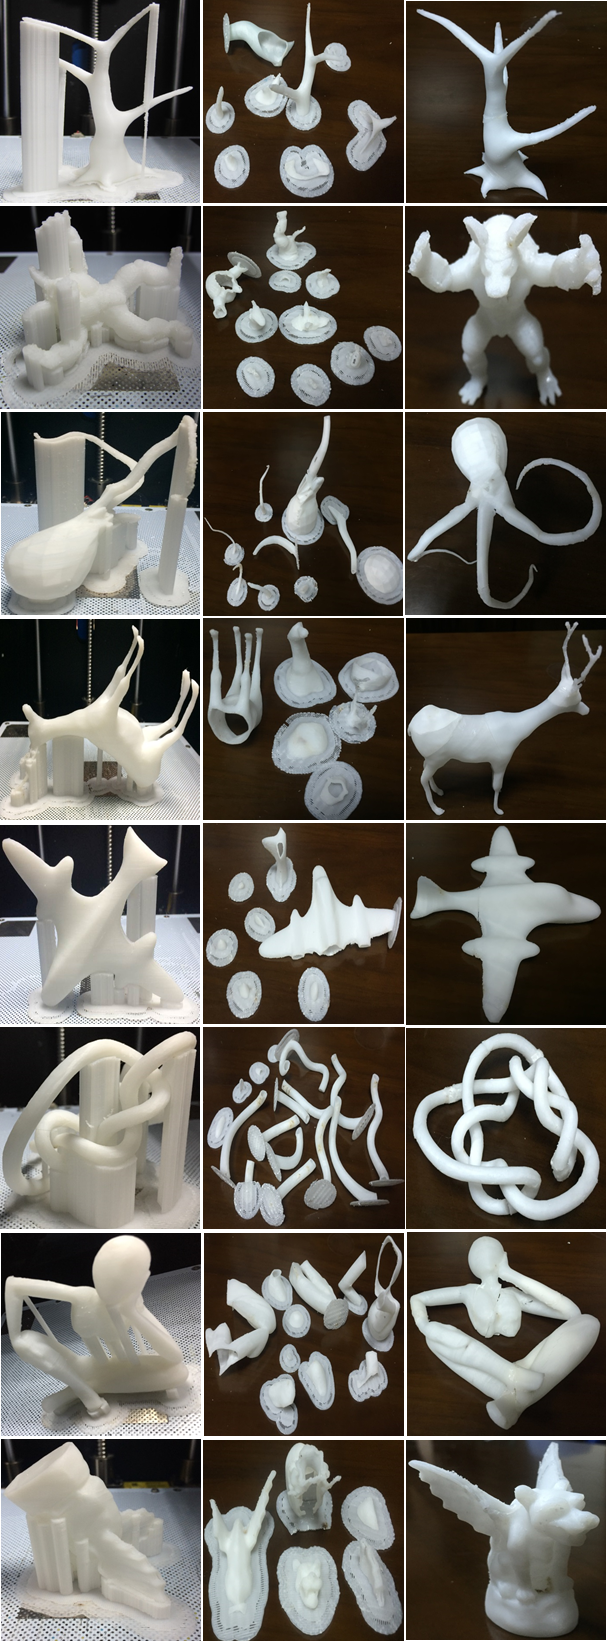
\includegraphics[width=0.975\linewidth]{figs/experiment.png}
  \caption{\label{fig:experiment}%
           A comparison between printing of original shell models and our partitioned models. The orientations of the models in the left column are determined as the optimal printing directions that correspond to the minimum amount of support materials (by using Meshmixer software provided by Autodesk). }
\end{figure}

%(iii) Currently, we set a connected flat region as the base of the a partition model, while in some cases it is possible that multiple connected flat regions on a plane served as the bases may lead to better partition result, but the determination of how many cuts and the positions of the cuts is even more intricate and is therefore a challenging future work.
